%20 min preso!
\documentclass[xcolor=table,aspectratio=169]{beamer}
\usepackage{beamerthemesplit}
\usepackage{wrapfig}
\usetheme{SPbGU}
\usepackage{pdfpages}
\usepackage{amsmath}
\usepackage{cmap}
\usepackage[T2A]{fontenc}
\usepackage[utf8]{inputenc}
\usepackage[english]{babel}
\usepackage{indentfirst}
\usepackage{amsmath}
\usepackage{tikz}
\usepackage{multirow}
\usepackage[noend]{algpseudocode}
\usepackage{algorithm}
\usepackage{algorithmicx}
\usepackage{fancyvrb}
\usetikzlibrary{calc}
\usetikzlibrary{shapes,arrows}
\usetikzlibrary{arrows,automata}
\usetikzlibrary{positioning}
\usetikzlibrary{fit}
%\usepackage{caption}
\usepackage{subcaption}

\usepackage{kbordermatrix}
\renewcommand{\kbldelim}{(} 
\renewcommand{\kbrdelim}{)}

\newcommand\mca{\multicolumn{1}{c}{\cellcolor{red}\textbf{\{a\}}}}
\newcommand\mcb{\multicolumn{1}{c}{\cellcolor{red}\textbf{\{b\}}}}

\usepackage{tabularx}
\newcolumntype{Y}{>{\raggedleft\arraybackslash}X}

\renewcommand{\thealgorithm}{}

\newtheorem{mytheorem}{Theorem}
\renewcommand{\thealgorithm}{}

\newcommand{\tikzmark}[1]{\tikz[overlay,remember picture] \node (#1) {};}
\def\Put(#1,#2)#3{\leavevmode\makebox(0,0){\put(#1,#2){#3}}}

\newcommand{\ltz}{$< 1$}


\tikzset{
    state/.style={
           rectangle,
           rounded corners,
           draw=black, very thick,
           minimum height=2em,
           inner sep=2pt,
           text centered,
           },
}

\beamertemplatenavigationsymbolsempty

\title[CFPQ In Terms of LA]{Context-Free Path Querying In Terms of Linear Algebra}
%\subtitle[YaccConstructor]{Parsing techniques for graph analysis}
% То, что в квадратных скобках, отображается в левом нижнем углу.
\institute[JetBrains Research]{
JetBrains Research, Programming Languages and Tools Lab  \\
Saint Petersburg University
}

% То, что в квадратных скобках, отображается в левом нижнем углу.
\author[Rustam Azimov]{\textbf{Rustam Azimov} \\ supervised by Semyon Grigorev }

\date{August 16, 2021}

\begin{document}
{
\begin{frame}[fragile]
  \begin{table}
  \centering
  \begin{tabularx}{\linewidth}{YcX}
    
\includegraphics[height=1.5cm]{pictures/jetbrainsResearch.pdf} \hfill
    & \begin{minipage}[t]{0.3\textwidth}\center \vspace{-1cm}  VLDB 2021 PhD Workshop
      \end{minipage}
    & \hfill 
\includegraphics[height=1.5cm]{pictures/SPbGU_Logo.png}
  \end{tabularx}
  \end{table}
  \titlepage
\end{frame}
}

\begin{frame} \frametitle{Context-Free Path Querying (CFPQ)}
  \begin{minipage}[m]{0.45\linewidth}
  \raisebox{-0.5\totalheight}{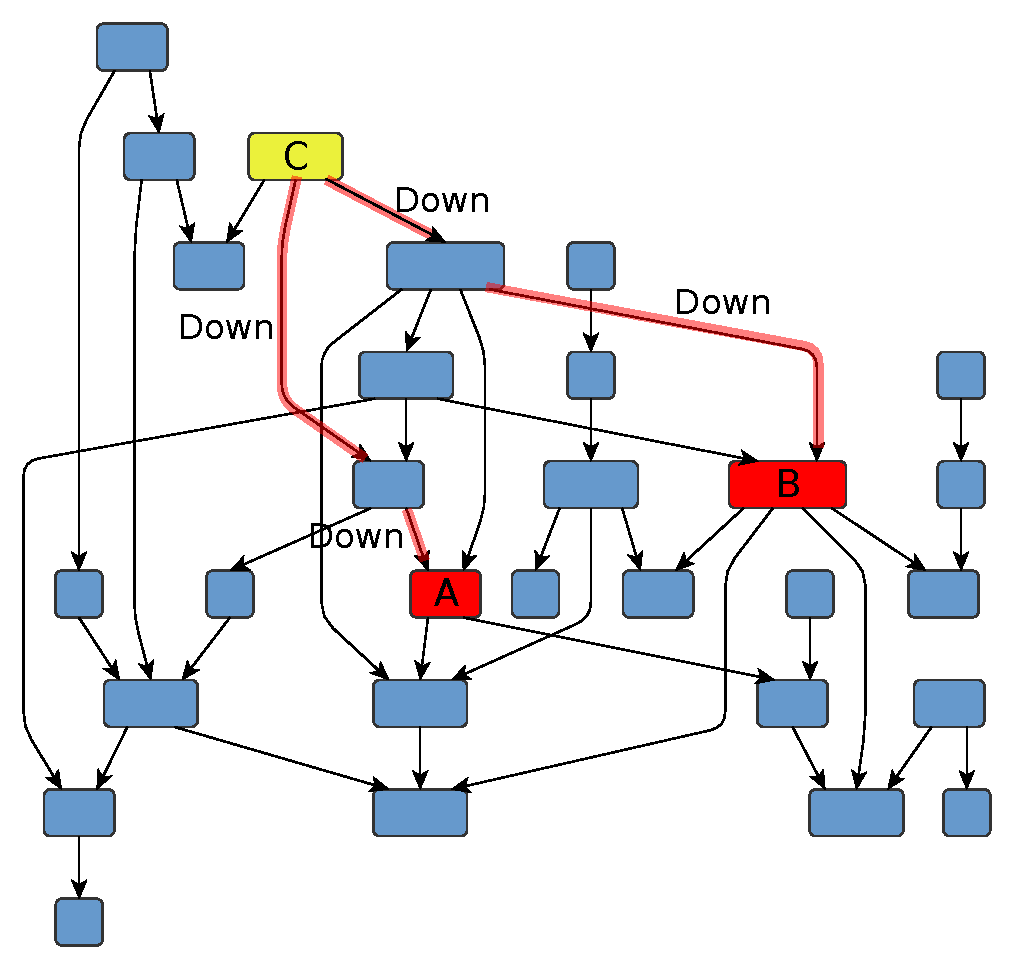
\includegraphics[width=\textwidth]{pictures/hierarchical.pdf}}
  \end{minipage}\hfill
  \begin{minipage}[m]{0.5\linewidth}
  \textbf{Context-free} languages as constraints on the paths
  \begin{itemize}
        \item Are nodes A and B on the same level of hierarchy?
        \item Is there a path of form $\overline{\textbf{Down}}^n \, \textbf{Down}^n$ between A and B?
        \item Find all paths of form $\overline{\textbf{Down}}^n \, \textbf{Down}^n$ between A and B
        
        \item Context-free grammar: $\textit{SameLvl} \to \overline{\textit{Down}} \ \textit{SameLvl} \ \textit{Down} \mid \varepsilon$
  \end{itemize}

  \end{minipage}

  \end{frame}

\begin{frame}[fragile]
	\frametitle{CFPQ}
	\begin{itemize}
		\item $L$ --- context-free language over the alphabet $\Sigma$
		\pause
		\item $G = (V,E,\Sigma')$ --- directed graph
		\begin{itemize}
			\item $v \xrightarrow{l} u \in E$
			\item $l \in 	\Sigma' \subseteq \Sigma$
		\end{itemize}
		\pause
		\item $\pi = v_0 \xrightarrow{l_0} v_1 \xrightarrow{l_1} \cdots \xrightarrow{l_{n-2}} v_{n-1} \xrightarrow{l_{n-1}} v_n$ --- path in $G$
		\item $\omega(\pi) = \omega(v_0 \xrightarrow{l_0} v_1 \xrightarrow{l_1} \cdots \xrightarrow{l_{n-2}} v_{n-1} \xrightarrow{l_{n-1}} v_n) = l_0 l_1 \cdots l_{n-1}$
		\pause
		\item It is necessary to find information about paths $\pi$, such that $\omega(\pi) \in L$
	\end{itemize}
\end{frame}

\begin{frame}[fragile] \frametitle{Formulations of the CFPQ Problem}
	\begin{itemize}
		\item type of the required information about paths in the graph \begin{itemize}
			\item solution of the reachability problem (relational query semantics)
			\item single path search (single-path query semantics)
			\item finding all paths in the graph (all-path query semantics)
		\end{itemize}
		\item fixing a set of source and destination vertices in the graph
		\begin{itemize}
			\item finding paths between all pairs of vertices (All-Pairs problem)
			\item a fixed set of source vertices (Multiple Source problem)
			\item single source single destination vertices
		\end{itemize}
		\item additional path constraints
		\begin{itemize}
			\item finding the shortest paths
			\item finding the simple paths
		\end{itemize}
	\end{itemize}
\end{frame}


  \begin{frame}[fragile] \frametitle{Applications}
    \begin{itemize}
      \item Static code analysis
       \begin{itemize}
      	\item interprocedural points-to analysis
      	\item interprocedural alias analysis
      \end{itemize}
      \item Graph database querying
      \item RDF analysis
      \item Bioinformatics
    \end{itemize}
  \end{frame}

\begin{frame}[fragile] \frametitle{Existing Solutions}
	\begin{itemize}
		\item Based on various parsing algorithms
		\begin{itemize}
			\item (G)LL and (G)LR-based algorithms% by Ciro M. Medeiros
			%et al., Fred C. Santos et al., Semyon Grigorev et al.,
			%and Ekaterina Verbitskaia et al.
			\item CYK-based algorithm% by Xiaowang Zhang et al.
			\item Combinators-based approach to CFPQ% by Ekaterina Verbitskaia et al.
		\end{itemize}
		\item Yet recent research by Jochem
		Kuijpers et al. shows that existing solutions are not applicable
		for real-world graph analysis because of significant
		\begin{itemize}
			\item running time
			\item memory consumption
		\end{itemize}
		\item Like with solutions of other graph analysis problems
		\begin{itemize}
			\item irregular access patterns lead to poor locality
			\item caching and parallelization are difficult
			\item limited portability after applying optimizations
		\end{itemize}
	\end{itemize}
\end{frame}

\begin{frame}[fragile] \frametitle{Linear Algebra (LA) For Graph Analysis Problems}
	\begin{itemize}
		\item The idea of using a sparse adjacency
		matrix as a graph representation in graph analysis problems
		is well-known
		\item Recently, became very popular the \textbf{GraphBLAS API} specification that defines standard building blocks for graph
		algorithms in the language of LA
		\item Using efficient libraries that implement it is a good recipe for making a high-performance parallel CFPQ
		solution if we can reduce the CFPQ problem to LA operations
		\begin{itemize}
			\item although such reduction was found for a number of graph
			algorithms (BFS, PageRank, Graph coloring, Connected components, \ldots)
			\item there are many graph algorithms for which it has not
			been done (DFS, \textbf{CFPQ}, \ldots)
		\end{itemize}
	\end{itemize}
\end{frame}

\begin{frame}[fragile] \frametitle{Research Statement}
	\begin{itemize}
		\item Aim: to explore the applicability of linear algebra methods to the CFPQ problem for obtaining the efficient implementations using parallel computations
		\item Objectives:
		\begin{itemize}
			\item An approach to solving the CFPQ problem using	LA methods will be provided
			\item Using provided approach, the CFPQ algorithms
			based on LA operations for relational, single-path,
			and all-path query semantics will be devised
			\item The efficient implementations of the devised algorithms
			for CFPQ evaluation using parallel computations will be provided, their experimental study on synthetic and real data will be conducted
		\end{itemize}
	\end{itemize}
\end{frame}


\begin{frame}[fragile] \frametitle{Proposed Approach}
		\centering
		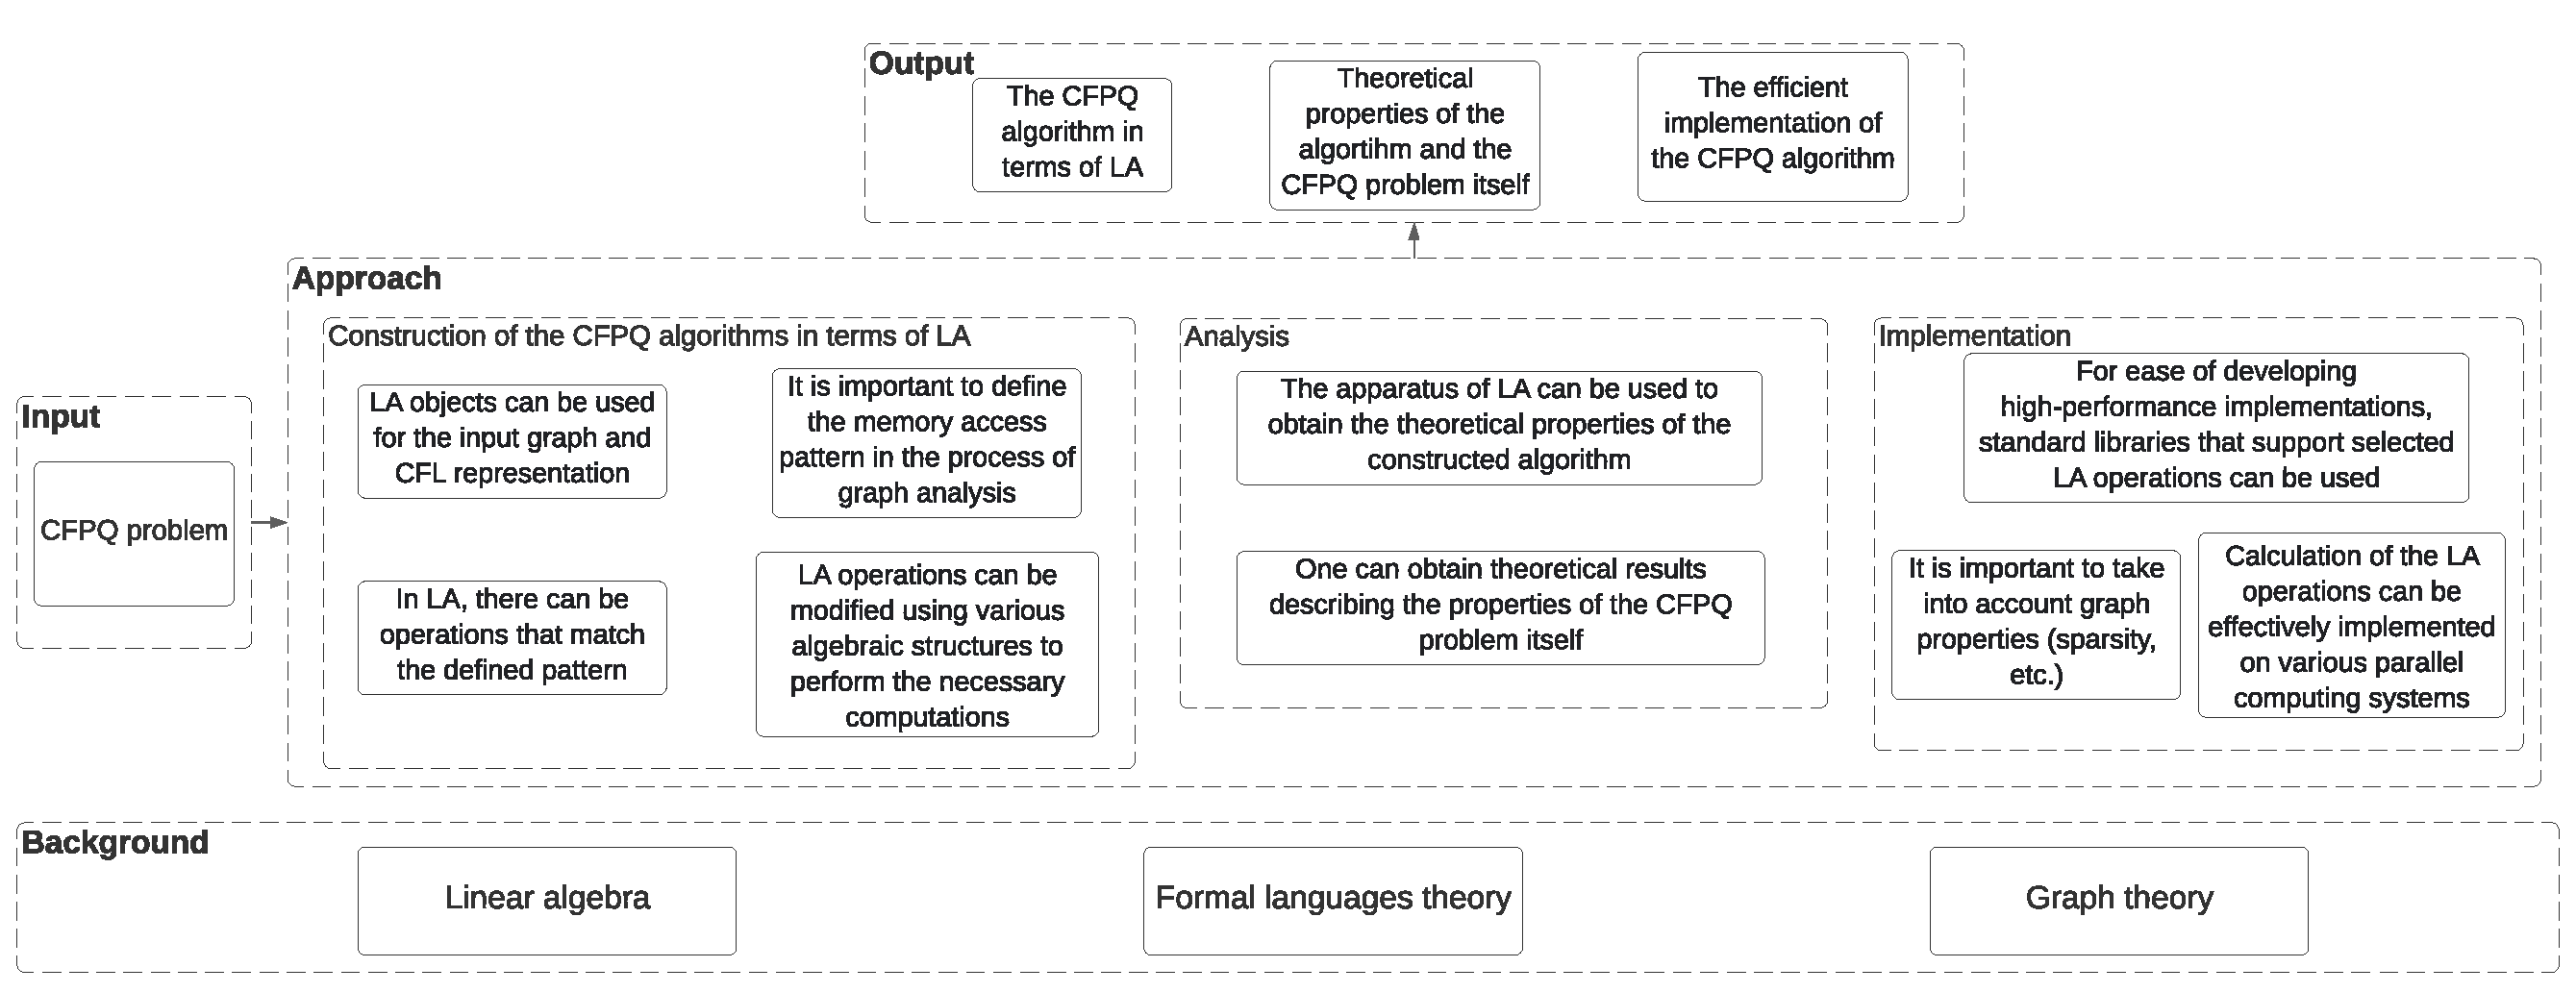
\includegraphics[width=15.7cm]{pictures/approach.pdf}
\end{frame}

\begin{frame}[fragile] \frametitle{Devised Algorithms: Matrix-Based}
	\begin{itemize}
		\item The all-pairs CFPQ algorithms for relational, single-path and all-path query semantics were devised
		\item Matrix-based CFPQ algorithms
		\begin{itemize}
			\item Represent the input graph using adjacency matrix
			\begin{itemize}
				\item boolean matrices for the relational query semantics	
				\item the additional information are stored for single-path and all-path query semantics
			\end{itemize}
			\item Use CF-grammars in normal form for describing the input CFL
			\item Construct the semirings for modifying the matrix multiplication operations
			\item Explore the graph by computing the transitive closure
			\item Resulting matrices are used for restoring found paths 
		\end{itemize}
	\end{itemize}
\end{frame}

  \begin{frame}[fragile] \frametitle{Matrix-Based Algorithm: Relational Query Semantics}
    	\begin{algorithm}[H]
    		\begin{algorithmic}[1]
    			\caption{Context-free path querying algorithm}
    			\label{lst:algo1}
    			\Function{evalCFPQ}{$D=(V,E,L), G=(\Sigma,N,P)$}
    			\State{$n \gets$ |V|}
    			\State{$T \gets \{T^{A_i} \mid A_i \in N, T^{A_i}$ is a matrix $n \times n$, $T^{A_i}_{k,l} \gets$ \texttt{false}\} }
    			\ForAll{$(i,x,j) \in E$, $A_k \mid A_k \to x \in P$}
    			%\Comment{Matrices initialization}
    			%\For{$A_k \mid A_k \to x \in P$}
    			{$T^{A_k}_{i,j} \gets \texttt{true}$}
    			%\EndFor
    			\EndFor
    			\ForAll{$A_k \mid A_k \to \varepsilon \in P$}
    			\ForAll{$i \in \{0,\ldots ,n-1\}$}
    			{$T^{A_k}_{i,i} \gets \texttt{true}$}
    			\EndFor
    			\EndFor
    			
    			\While{any matrix in $T$ is changing}
    			%\Comment{Transitive c	losure calculation}
    			\For{$A_i \to A_j A_k \in P$}
    			{ $T^{A_i} \gets T^{A_i} + (T^{A_j} \times T^{A_k})$ } 
    			\EndFor
    			\EndWhile
    			\State \Return $T$
    			\EndFunction
    		\end{algorithmic}
    	\end{algorithm}
  \end{frame}

\begin{frame}[fragile] \frametitle{Devised Algorithms: Kronecker Product-Based}
	\begin{itemize}
		\item On the contrary, the algorithms in the second group are based on the Kronecker product operation
		\begin{itemize}
			\item Do not require the transformation of the CF-grammar
			\begin{itemize}
				\item The transformation to Chomsky normal form leads to at least a quadratic blow-up in grammar	size
			\end{itemize}
			\item Use Recursive State Machines (RSMs) for describing the input CFL
			\begin{itemize}
				\item The RSMs can be represented as graphs
			\end{itemize}
			\item Evaluate query using the Kronecker product of the corresponding adjacency matrices of the input graph and the RSM
		\end{itemize}
	\end{itemize}
\end{frame}

\begin{frame}[fragile] \frametitle{Implementations}

\begin{itemize}
	\item For evaluation we use the following CPU-based implementations of CFPQ algorithms based on the GraphBLAS API and sparse matrix representation
	\begin{itemize}
		\item \textbf{$MtxRel$} --- the matrix-based implementation for  relational query semantics
		\item \textbf{$MtxSingle$} --- for  single-path query semantics
		\item \textbf{$MtxAll$} --- for all-path query semantics
		\item \textbf{$Tns$} --- the implementation of the Kronecker product-based algorithm for all-path query semantics
		
	\end{itemize}
\end{itemize}
\end{frame}


\begin{frame} \frametitle{Evaluation Setup}
  \begin{itemize}
  	\item Ubuntu 18.04, Intel Core i7-6700 CPU, 3.4GHz, DDR4 64Gb RAM
  	\item We use graphs corresponding to real RDFs
  	\item We use same-generation query
  \end{itemize}
\end{frame}

\begin{frame}[fragile] \frametitle{Evaluation: CFPQ\footnote{Time in seconds and memory is measured in megabytes}}
\begin{center}
	\tikzmark{yyy}{
	}
	{\scriptsize
	{\setlength{\tabcolsep}{0.3em}
			\rowcolors{3}{}{lightgray}
					\begin{tabular}{|l|l|l|l|l|l|l|l|l|l|l|}
						\hline
						\multicolumn{1}{|c|}{\multirow{2}{*}{Graph}} & \multicolumn{1}{c|}{\multirow{2}{*}{\#V}} & \multicolumn{1}{c|}{\multirow{2}{*}{\#E}} &  \multicolumn{2}{c|}{MtxRel} & \multicolumn{2}{c|}{MtxSingle} & \multicolumn{2}{c|}{MtxAll} & \multicolumn{2}{c|}{Tns} \\ \cline{4-11} 
						\multicolumn{1}{|c|}{}                       & \multicolumn{1}{c|}{}                     & \multicolumn{1}{c|}{}                     & Time         & Mem          & Time        & Mem        & Time           & Mem           & Time         & Mem    \\ \hline
						pathways                                     & 6 238                                     & 18 598 & 0.01         & 140  & 0.01           & 671 & 0.01         & 49           & 0.01        & 122               \\ \hline
						go-hierarchy                                 & 45 007                                    & 980 218                                   & 0.09         & 255 & 0.84           & 671 & 0.35        & 195        & 0.24        & 252                             \\ \hline
						enzyme                                       & 48 815                                    & 109 695                                   & 0.01         & 181 & 0.01           & 217 & 0.02         & 61           & 0.02        & 132                            \\ \hline
						eclass\_514en                                & 239 111                                   & 523 727                                   & 0.06         & 181 & 0.16           & 216    & 0.22         & 126          & 0.27        & 193                         \\ \hline
						go                                           & 272 770                                   & 534 311                                   & 0.94         & 246  & 0.93           & 217  & 1.13         & 990          & 1.27        & 243                          \\ \hline
						%geospecies                                   & 450 609                                   & 2 311 461                   & 0.01         & 248 & 0.01           & 2251            & 0.34         & 156          & 0.01        & 196              \\ \hline
						geospecies & 450 609                                   & 2 311 461 & 7.48         & 7645     & 15.54          & 22941 & 32.06        & 44235        & 26.32       & 19537 \\ \hline
						taxonomy                                     & 5 728 398                                 & 14 922 125                            & 0.72         & 1175      & 1.15           & 2250    & 3.84        & 1507        & 3.56        & 1776                   \\ \hline
					\end{tabular}
	}
}
 \end{center}
\pause
\onslide<2>{\tikz[overlay,remember picture]{\draw[draw=red,thick,fill opacity=0.2] ($ (yyy) + (5.22,-0.41)$) rectangle ($ (yyy) + (8.78,-1.53)$);}}
\pause
\onslide<3>{\tikz[overlay,remember picture]{\draw[draw=red,thick,fill opacity=0.2] ($ (yyy) + (6.88,-0.41)$) rectangle ($ (yyy) + (10.58,-1.53)$);}}
\pause
\onslide<4>{\tikz[overlay,remember picture]{\draw[draw=red,thick,fill opacity=0.2] ($ (yyy) + (8.69,-0.41)$) rectangle ($ (yyy) + (12.40,-1.53)$);}}
\end{frame}

\begin{frame}[fragile] \frametitle{Evaluation: Average Path Extraction Time For \textit{go}}
\begin{center}
    \[
		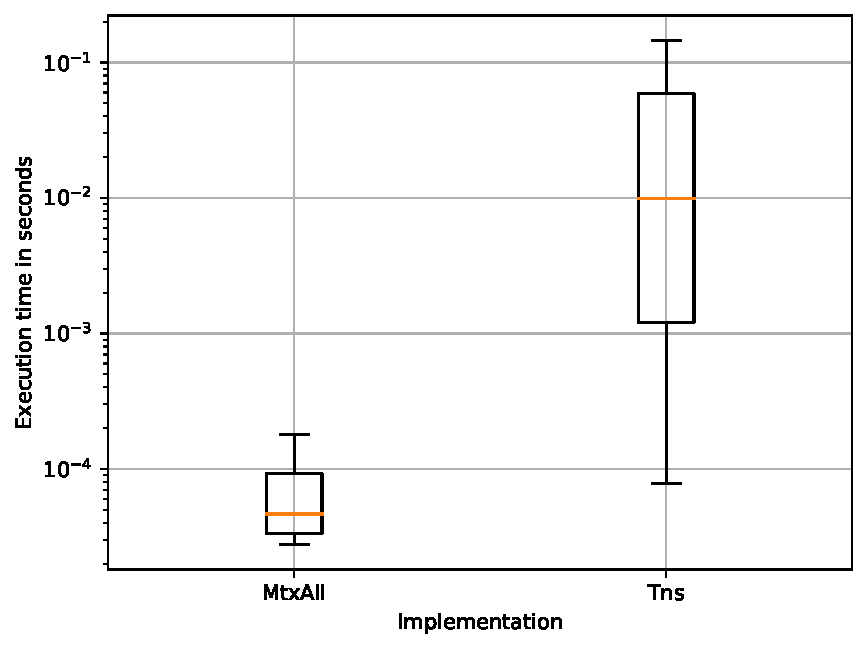
\includegraphics[width=9cm]{pictures/go_10_all_matrixall_tensor.pdf}
	\]
\end{center}

\end{frame}

\begin{frame}[fragile] \frametitle{Preliminary Results}
	\begin{itemize} 
		\item The single-path matrix-based algorithm constructs matrices up to 2 times slower than the relational matrix-based algorithm
		\item The all-path matrix-based algorithm constructs matrices up to 2-3 times slower than the single-path matrix-based algorithm
		\pause
		\item If it is necessary to frequently recalculate
		the matrices for a changing graph or a path query then the best
		choice is the Kronecker product-based algorithm with
		faster and less memory consuming matrices construction
		\pause
		\item If it is  necessary to extract paths many times for a once constructed
		matrices or matrix changes can be efficiently computed dynamically then the proposed matrix-based CFPQ algorithm is  preferable
	\end{itemize}
	%\pause
	%\begin{itemize}
	% \item Dataset is published: both graphs and queries
	%\begin{itemize}
	%	\item Link: \url{https://github.com/JetBrains-Research/CFPQ_Data}
	%\end{itemize}
	
	%\item Implementations are available on GitHub
	%\begin{itemize}
	%	\item Link: \url{https://github.com/JetBrains-Research/CFPQ_PyAlgo}
	%\end{itemize}
	
	%\end{itemize}
\end{frame}

\begin{frame}[fragile] \frametitle{Conclusion}
  \begin{itemize}
    \item We provide an approach to solving the CFPQ
    problem using LA methods that allows one to get interesting practical and theoretical results
    \pause
    \item Using provided approach we devise the CFPQ algorithms for all three query semantics based on such LA operations as matrix multiplication and Kronecker product
    \pause
    \item We provide the efficient implementations of the devised algorithms using the implementations of the GraphBLAS API with parallel computations and sparse matrix representations
    \pause
    \item We can conclude that the devised LA-based CFPQ solutions are applicable for real-world graph analysis
  \end{itemize}
  %\pause
  %\begin{itemize}
   % \item Dataset is published: both graphs and queries
    %\begin{itemize}
    %	\item Link: \url{https://github.com/JetBrains-Research/CFPQ_Data}
    %\end{itemize}
    
    %\item Implementations are available on GitHub
    %\begin{itemize}
    %	\item Link: \url{https://github.com/JetBrains-Research/CFPQ_PyAlgo}
    %\end{itemize}
    
  %\end{itemize}
\end{frame}

\begin{frame}[fragile] \frametitle{Publications and Conferences}
	\begin{enumerate}
		\item Context-Free Path Querying by
		Matrix Multiplication / Azimov R., Grigorev S. (GRADES-NDA’18)
		\item Context-Free Path Querying with Single-Path Semantics by
		Matrix Multiplication / Terekhov A., Khoroshev A., Azimov R., Grigorev S. (GRADES-NDA’20)
		\item Context-Free Path Querying by Kronecker
		Product / Orachev E., Epelbaum I., Azimov R., Grigorev S. (ADBIS’20)
		\item Context-Free Path Querying with All-Path Semantics by
		Matrix Multiplication / Azimov R., Epelbaum I., Grigorev S. (GRADES-NDA’21)
		
		\item Context-Free Path Querying In Terms of Linear Algebra / Azimov R. (VLDB-PhD'21)
	\end{enumerate}
\end{frame}

\begin{frame}[fragile] \frametitle{Future Research}
  \begin{itemize}
  	\item As a next step, we plan to provide a full comparison of our LA-based implementations with all state-of-the-art CFPQ solutions on the same benchmark and experimental setup
  	\item We compare the CPU-based implementation. In the future, we
  	want to obtain GPU-based and distributed implementations for all devised algorithms
    \item Also, we plan to provide the multiple-source
    modifications for all LA-based CFPQ algorithms
\end{itemize}
\end{frame}

\begin{frame}
\frametitle{Contact Information}
\begin{itemize}
  \item Rustam Azimov:
  \begin{itemize}
  	\item \href{mailto:rustam.azimov19021995@gmail.com}{rustam.azimov19021995@gmail.com}
  	\item \href{mailto:Rustam.Azimov@jetbrains.com}{Rustam.Azimov@jetbrains.com}
  \end{itemize}
\item Semyon Grigorev:
\begin{itemize}
	\item \href{mailto:s.v.grigoriev@spbu.ru}{s.v.grigoriev@spbu.ru}
	\item \href{mailto:Semen.Grigorev@jetbrains.com}{Semen.Grigorev@jetbrains.com}
\end{itemize}
\vspace{0.5cm}
  \item Dataset: \href{https://github.com/JetBrains-Research/CFPQ_Data}{https://github.com/JetBrains-Research/CFPQ\_Data}
   \item Algorithm implementations: \href{https://github.com/JetBrains-Research/CFPQ_PyAlgo}{https://github.com/JetBrains-Research/CFPQ\_PyAlgo}
\end{itemize}
\vspace{0.1cm}
\center{\huge{Thanks!}}
\end{frame}
\end{document}
